\documentclass[10p]{beamer}
\usepackage[utf8]{inputenc}
\usepackage{graphicx}
\usepackage{perso}
\usepackage{animate}

\usetheme{Warsaw}
\setbeamerfont{block body}{size=\small}
\setbeamerfont{block body alerted}{size=\small}
\date{}
\AtBeginSubsection[]
{
  \begin{frame}
  \frametitle{Sommaire}
  \tableofcontents[currentsubsection]
  \end{frame} 
}
\title{New clustering methods into a parallel code}
\author[SORIANO, AUBENEAU, DUVAL, PRIEUL, SANTINA]{SORIANO Tristan, AUBENEAU Simon, DUVAL Quentin, PRIEUL Simon, SANTINA Jeremy}
\institute{ENSEEIHT, 3IN}
\begin{document}
\begin{frame}
\maketitle
\end{frame}
\section{Introduction}
\begin{frame}
\frametitle{Clustering method}
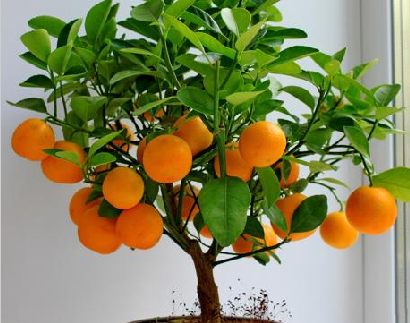
\includegraphics[width=0.5\textwidth]{Image/Oranger.png}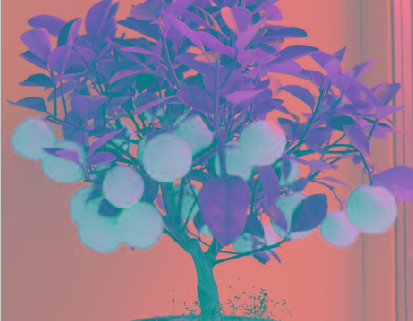
\includegraphics[width=0.5\textwidth]{Image/OrangerClust.png}
\end{frame}
\begin{frame}
\frametitle{High computational complexity}
\begin{columns}
\begin{column}{0.4\textwidth}
\begin{itemize}
\item Huge quantity of data
\item Dense matrices
\item Extended applications
\end{itemize}
\end{column}
\begin{column}{0.6\textwidth}
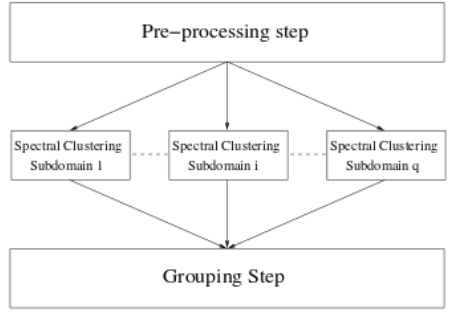
\includegraphics[width=\columnwidth]{Image/parallel.png}
\end{column}
\end{columns}
\end{frame}
\section{Work organisation}
\subsection{Project management}
\begin{frame}
\small
\frametitle{Development Plan}
\begin{description}
\item [Step 1] Theoritical study + Matlab new methods implementation
\item [Step 2] Code documentation + Fortran interfaces specification
\item [Step 3] Code refactoring + Fortran implementation
\item [Step 4] Validation
\end{description}
\tiny
\begin{tabular}{|l|l|l|l|}
\hline
\textbf{Risk Description} & \textbf{Probability} & \textbf{Impact} & \textbf{Action}
\\
\hline
Unsatisfied client & Light & Heavy & Specification with the client
\\
\hline
Unsuitable ressources & Medium & Heavy & Lighter test creation, early access request
\\
\hline
Insufficient knowledge & Heavy & Medium & Increase the time dedicated to each risky task
\\
\hline
\end{tabular}
\end{frame}
\begin{frame}
\frametitle{Team organization}
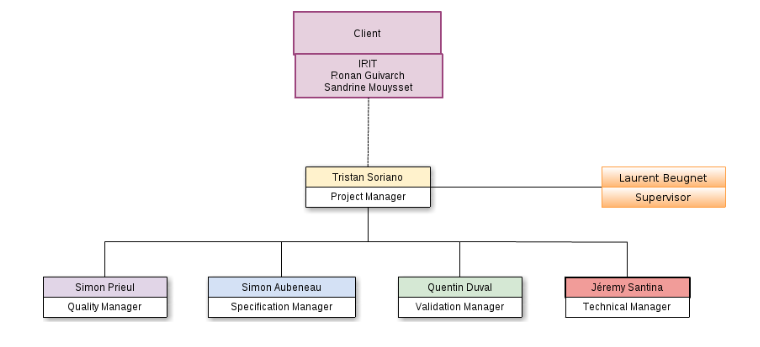
\includegraphics[width=\textwidth]{Image/organisation.png}
\end{frame}
\begin{frame}
\frametitle{Technologies}

\includegraphics[width=\textwidth]{Image/logos.png}
\end{frame}
\subsection{Starting point}
\begin{frame}
\frametitle{Configuration}
\begin{itemize}
\item Makefile for specific environment
\item Libraries:
\begin{itemize}
\item MPI
\item Lapack
\item Arpack
\end{itemize}
\item F90 compilator (gfortran, ifort…)
\item Makefile.x has to specify the correct paths of the libraries above
\end{itemize}
\end{frame}
\section{Reverse engineering}
\subsection{Doxygen documentation}
\begin{frame}
\frametitle{Autogeneration with Doxygen}
\begin{block}{Detected features}
\begin{itemize}
\item \textbf{Modules and programs} : name
\item \textbf{Routines} : name and parameters
\item \textbf{Parameters} : name and type
\end{itemize}
\end{block}
\begin{block}{Produced output formats}
\begin{itemize}
\item \textit{HTML}: Documentation readable by a web browser
\item \textit{PDF}: Documentation written in LaTex to generate a PDF file
\end{itemize}
\end{block}
\end{frame}

\begin{frame}[fragile,allowframebreaks]
\frametitle{Specific comments}
\begin{block}{Useful keywords}
\begin{itemize}
\item \textbf{@details} \textit{text}: detailed description of a module, structure or method
\item \textbf{@param} \textit{name} [\textit{dir}] \textit{text}: description of a parameter 
\end{itemize}
\end{block}
\begin{example}
\begin{lstlisting}
!> Puts the index number of the pixels into an array.
!! @details Each point of the data set is mapped to 
!! an array corresponding to an image. Two indices 
!! will be used (row and column) instead of one.
!! @note the data set has to be in picture format.
!! @param[in,out] data the data set
SUBROUTINE assign_picture_array(data)
\end{lstlisting}
\end{example}

\begin{alertblock}{Remarks}
\begin{enumerate}
\item Documentation depends on refactoring
\item Most of the parameters are similar from one method to another
\item It is an highly repetitive work
\end{enumerate}
\end{alertblock}
\begin{block}{Automated comments writing}
\begin{itemize}
\item Descriptions in tables in a MySQL Database
\item Software in Java for writing specific comments
\end{itemize}
\end{block}
\end{frame}
\subsection{Code refactoring}
\begin{frame}
\frametitle{Changing source code}
\begin{block}{Purpose}
Improve software quality and portability
\end{block}
\begin{enumerate}
\item Changing the types "REAL" and "REAL(KIND=*)" into "DOUBLE PRECISION" and "INTEGER(KIND=*)" into "INTEGER"
\item Changing the types "CHARACTER*x" into "CHARACTER (LEN=x)"
\item Changing the types of some “INTEGER” variables used as boolean into “LOGICAL”
\end{enumerate}
\end{frame}
\begin{frame}
\frametitle{Organising source code}
\begin{block}{Purpose}
Improve readability and maintainability of the code
\end{block}
\begin{enumerate}
\item Fortran keywords transformed in UPPERCASE
\item Removing of the commented code
\item Declarations of parameters and variables at the beginning of a subroutine or program : one declaration line, ordered by type and name
\item Removing the semicolons : only one instruction per line
\item Removing the unused variables
\end{enumerate}
\end{frame}
\begin{frame}
\frametitle{Renaming and translating}
\begin{block}{Purpose}
Improve readability and internationalization
\end{block}
\begin{enumerate}
\item Translation of the comments helping the understanding of the code
\item Rename methods : standardization (underscore to separate the different words), translation in english, better naming, blank space after each comma in the signature, blank space after each comma in the signature
\item Rename parameters of methods and variables : standardization (underscore to separate the different words), translation in english, better naming
\item Translation of all the “PRINT” messages (displayed in the console during execution)
\end{enumerate}
\end{frame}
\section{Clustering algorithms}
\subsection{Spectral Clustering}
\begin{frame}
\frametitle{Description}
\begin{block}{Main idea}
Create a pounded graph between points
\end{block}
\vfill
\begin{columns}
\begin{column}{0.6\textwidth}
\begin{itemize}
\item Each vertice weight represents the similarity between points
\item The final graph is cut on the lowest similarity vertices
\end{itemize}
\end{column}
\begin{column}{0.4\textwidth}
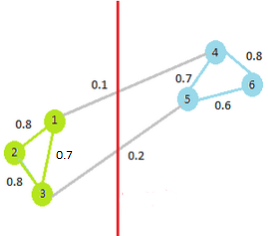
\includegraphics[width=\columnwidth, height=4cm]{Image/graph.png}
\end{column}
\end{columns}
\end{frame}
\subsection{Kernel-K-Means}
\begin{frame}
\frametitle{K-Means}
\begin{block}{Main idea}
Select random centers for cluster and move them until they reach centers of density.
\end{block}
\begin{columns}
\begin{column}{0.6\textwidth}
\begin{enumerate}
\item Find minimum distances to cluster centers
\item Compute density centers
\item Select new cluster centers
\item Continue until cluster centers and density centers are similar
\end{enumerate}
\end{column}
\begin{column}{0.4\textwidth}
\animategraphics[autoplay,loop,width=\columnwidth]{1}{Image/kmeans}{1}{7}
\end{column}
\end{columns}
\end{frame}
\begin{frame}
\frametitle{Description}
\begin{block}{Main idea}
Enhance K-Means algorithm using a Kernel function to map the original points to a feature space.
\end{block}
\begin{center}
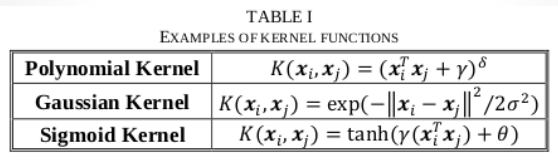
\includegraphics[width=0.5\textwidth]{Image/kernel.png}
\end{center}
\end{frame}
\subsection{Mean Shift}
\begin{frame}
\frametitle{Description}
\begin{block}{Main idea}
Move a window over the data set following the density gradient.
\end{block}
\begin{columns}
\begin{column}{0.6\textwidth}
\begin{enumerate}
\item Compute the mean of density in the specified window
\item Compute difference between center of the window and computed mean
\item Select the computed mean as the new center of the window
\item Restart until difference close to 0
\end{enumerate}
\end{column}
\begin{column}{0.4\textwidth}
\animategraphics[autoplay,loop,width=\columnwidth]{1}{Image/meanshift}{1}{6}
\end{column}
\end{columns}
\end{frame}
\subsection{Results}
\begin{frame}

\end{frame}
\section{Conclusion}
\begin{frame}
\end{frame}
\end{document}